% !TEX root = ./main.tex
%%%%%%%%%%%%%%%%%%%%%%%%%%%%%%%%%%%%%%%%%%%%%%%%%%%%%%%%%%%%%%%%%%%%%%%%%%%%%%%%%%%%%%%%%%
% Dans cette section, vous devez étudier complètement la complexité de votre code.       %
% Soyez le plus formel (i.e., mathématique) possible.                                    %
%%%%%%%%%%%%%%%%%%%%%%%%%%%%%%%%%%%%%%%%%%%%%%%%%%%%%%%%%%%%%%%%%%%%%%%%%%%%%%%%%%%%%%%%%%
\section{Complexité}\label{complexite}
%%%%%%%%%%%%%%%%%%%%
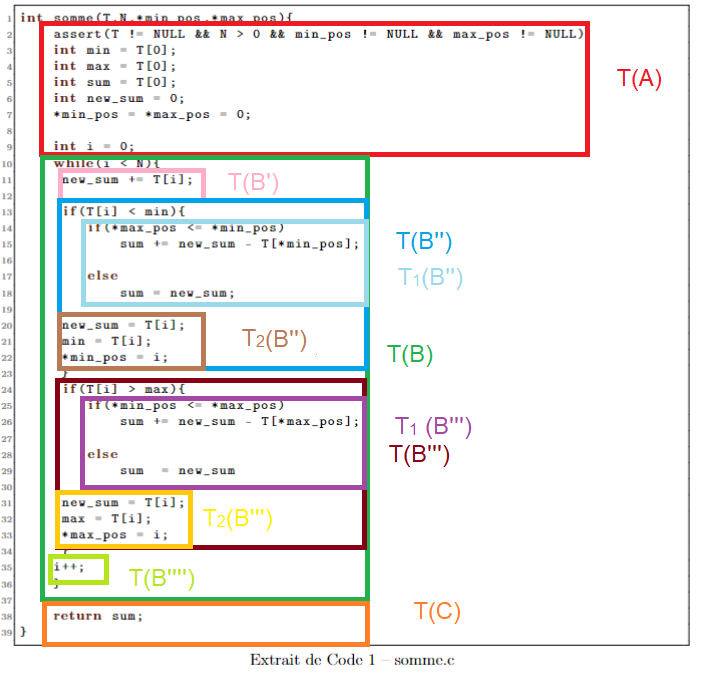
\includegraphics[width = 15 cm]{complexite.png}
\begin{enumerate}
    \item[-] Par application des règles 2 et 6 : 
    \[T(N) = T(A) + T(B) + T(C)\]
    \item[-] Par application des règles 1 et 5 : 
    \[T(N) = 8 + \sum_{i = 0}^{N-1} {(T(B') + T(B'') + T(B''') + T(B''''))} + 1\]
    \[T(N) = 8 + \sum_{i = 0}^{N-1} {(1 + T(B'') + T(B''') + 1)} + 1\]
    \item[-] Quid de T(B'') ? 
    \[T(B'') = T_1(B'') + T_2(B'')\]
    \item[-] Quid de $T_1$ (B'') ? Par application de la règle 3 :
    \[T_1(B'') = max(T_{if}(), T_{else}())\]
    \[T_{if}() = 1\] et \[T_{else}() = 1\] donc
    \[T_1(B'') = 1\]
    \item[-] Quid de $T_2$(B'') ? Par application de la règle 2 :
    \[T_2(B'') = 3\]
    \item[-] Ainsi T(B'') devient : 
    \[T(B'') = 1 + 3\]
    \[T(B'') = 4\]
    \item[-] Quid de T(B''') ?
    \[T(B''') = T_1(B''') + T_2(B''')\]
    \item[-] Quid de $T_1$(B''') ? Par application de la règle 3:
    \[T_1(B''') = max(T_{if}(), T_{else}())\]
    \[T_{if}() = 1\] et \[T_{else}() = 1\] donc
    \[T_1(B''') = 1\]
    \item[-] Quid de $T_2$(B''') ? Par application de la règle 2 :
    \[T_2(B''') = 3\]
    \item[-] Ainsi T(B''') devient : 
    \[T(B''') = 1 + 3\]
    \[T(B''') = 4\]
    \item[-] Ainsi T(B) devient : 
    \[\[T(B) = \sum_{i = 0}^{N-1} {10} = 10N\]\]
    \item[-] Donc:
    \[T(N) = 8 + 10N + 1 = 9 + 10N\]
    \item[-] Par quoi borner T(N) ?
    \[O(n)\] complexité linéaire.
\end{enumerate}
Preuve ?\\\indent
But : Trouver une constante \textit{c} $\in \math{R^+}$ et un seuil $n_0$ à partir duquel $T(n_0)$ $\leq$ $c$ x $n_0$.
\\\indent On remarque que pour $c = 11$ et $n_0$ = 9 on a $\forall n \geq n_0$: c x n $\geq$ 9 + 10N\\
\underline{exemple:}\begin{enumerate}
    \item[-] si n = 9 : 99 $\geq$ 99
    \item[-] si n = 10 : 110 $\geq$ 109
    \item[-] si n = 11 : ...
\end{enumerate}